\documentclass{xjtureport}
\usepackage{listings}
\usepackage{ctex}
\usepackage{graphicx}
\usepackage{xcolor}
\usepackage{subfigure}
\usepackage{parskip}
% author:wanghaixiang
\lstset{language=bash, numbers=left, numberstyle=\tiny, keywordstyle=\color{blue!70},}
% \lstset{
%     basicstyle          =   \sffamily,          % 基本代码风格
%     keywordstyle        =   \bfseries,          % 关键字风格
%     commentstyle        =   \rmfamily\itshape,  % 注释的风格,斜体
%     stringstyle         =   \ttfamily,  % 字符串风格
%     flexiblecolumns,                % 别问为什么,加上这个
%     numbers             =   left,   % 行号的位置在左边
%     showspaces          =   false,  % 是否显示空格,显示了有点乱,所以不现实了
%     numberstyle         =   \zihao{-5}\ttfamily,    % 行号的样式,小五号,tt等宽字体
%     showstringspaces    =   false,
%     captionpos          =   t,      % 这段代码的名字所呈现的位置,t指的是top上面
%     frame               =   lrtb,   % 显示边框
% }

\lstdefinestyle{cpp}{
    language        =   cpp, % 语言选Python
    basicstyle      =   \zihao{-5}\ttfamily,
    numberstyle     =   \zihao{-5}\ttfamily,
    keywordstyle    =   \color{blue},
    keywordstyle    =   [2] \color{teal},
    stringstyle     =   \color{magenta},
    commentstyle    =   \color{red}\ttfamily,
    breaklines      =   true,   % 自动换行,建议不要写太长的行
    columns         =   fixed,  % 如果不加这一句,字间距就不固定,很丑,必须加
    basewidth       =   0.5em,
    }
\definecolor{codegray}{rgb}{0.5,0.5,0.5}
\definecolor{backcolour}{rgb}{0.95,0.95,0.92}

\lstdefinestyle{whx}{
    backgroundcolor=\color{backcolour},
    commentstyle=\color{codegray},
    keywordstyle=\color{blue},
    numberstyle=\tiny\color{codegray},
    stringstyle=\color{red},
    basicstyle=\ttfamily\footnotesize,
    breakatwhitespace=false,
    breaklines=true,
    captionpos=b,
    keepspaces=true,
    numbers=left,
    numbersep=5pt,
    showspaces=false,
    showstringspaces=false,
    showtabs=false,
    tabsize=2
}
% \lstset 是对库进行设置,主要是设置某些关键的地方,它含有很多字段;
% \lstdefinestyle{Python} 是新定义一个叫做Python的样式,到时候直接引用这个设置就可以;
% \lstset 和 \lstdefinestyle{Python} 的东西差不多,不同之处就是优先级不同,后者更高,
% 前者是在你没有在 Python 中进行相关设定的时候,为你自动设置的一些东西。
% 总而言之,Python 样式里有的,一定会在 Python 代码里忠实被执行;Python 样式里没有的,系统会检查 \lstset 里有没有相关设置,如果有就用,没有的话就用系统的默认设置。
% =============================================
% Part 0 Edit the info
% =============================================

\major{人工智能}
\name{王海翔}
\title{本科实验报告}
\stuid{2203312479}
\college{电子与信息学部}
\date{\zhtoday}
\lab{科学馆203}
\course{机器人导航实验}
\instructor{张唐一可}
\grades{}
\expname{机器人导航控制实验}
\exptype{仿真实验}
\partner{}

\begin{document}
% =============================================
% Part 1 Header
% =============================================
\makecover
\makeheader
% =============================================
% Part 2 Main document
% =============================================

\section{实验目的和要求}
\subsection{实验目的}
轨迹跟踪是指根据某种控制理论,为机器人系统设计一个循迹控制器,使机器人能够到达并最终以期望的速度跟踪期望轨迹。
控制系统的任务即是严格按照这个参考路径(以及速度等控制输入量)去控制机器人运动。
本实验旨在通过机器人控制实验,使同学们掌握无人驾驶横纵向控制的基本方法,
培养和提高同学们应用控制理论解决实际问题的能力。

\subsection{实验要求}
实现基于PID的机器人循迹控制。
\begin{enumerate}
    \item 掌握实验原理并绘制主要模块框图。
    \item 针对不同的算法进行性能分析。
    \item 提出改善控制性能的可行方案。
\end{enumerate}
\section{实验环境}
\subsection{硬件环境}
dell Optiplex 7070 /i7-9700/32G/2T+256GSSD/DVD刻录/NVIDIA GeForce GTX 1650, 4GB
\subsection{软件环境}
\begin{enumerate}
    %cat /proc/version
    \item 操作系统:Ubuntu 18.0.4
    \item Python:3.7.3
    \item ROS1:Melodic
\end{enumerate}

\section{实验内容}
\begin{enumerate}
    \item 实现基于PID的循迹控制器。
    \item 实现模糊自适应PID控制
    \item 实现模型预测控制(MPC)可选
\end{enumerate}

\section{实验原理}
\subsection{算法概述}
PID算法是一种常用的控制算法,它可以通过对被控对象输出和目标值之间的误差进行计算,来实现对被控对象的精确控制。PID算法由比例控制(P)、积分控制(I)和微分控制(D)三个部分组成。

具体地说,PID控制器的输出$u(t)$是由三个部分组成的加权和:

$$u(t) = K_{p}e(t) + K_{i}\int_{0}^{t}e(\tau)d\tau + K_{d}\frac{de(t)}{dt}$$

其中,$e(t)$表示目标值与被控对象输出之间的误差,$K_p$、$K_i$和$K_d$分别表示比例系数、积分系数和微分系数。

具体如下流程图:
\begin{figure}[H]
    \centering
    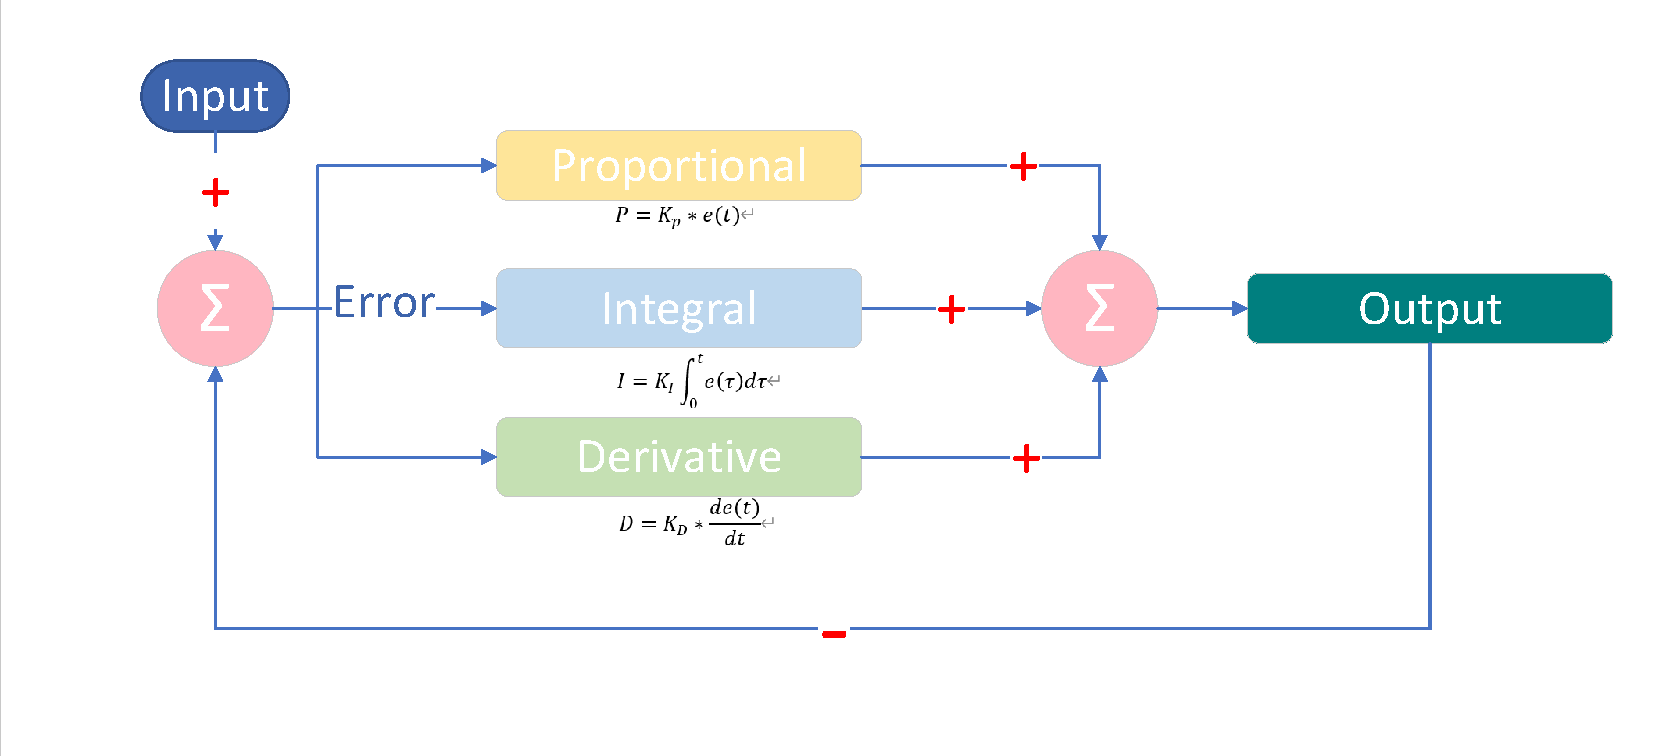
\includegraphics[width=18cm]{figures/PID流程图.pdf}
    \caption{PID流程图}
    \label{fig:PID流程图}
\end{figure}
其中,输入为Input,输出为Output即为u(t)

比例控制器$P$的作用是根据误差的大小来控制输出,它可以让被控对象快速地接近目标值。但是,由于比例控制器无法消除误差,因此在误差较大时,它的输出会产生较大的波动。

积分控制器$I$的作用是消除误差,它可以根据误差的积分值来控制输出,从而消除误差。但是,积分控制器会导致系统产生较慢的响应,并可能引起系统的不稳定性。

微分控制器$D$的作用是根据误差的变化率来控制输出,它可以提高系统的稳定性并消除瞬态误差。但是,微分控制器对噪声和干扰非常敏感,因此需要谨慎使用。

通过对比例、积分和微分控制器的加权和进行控制,PID控制器可以同时兼顾快速响应、消除误差和稳定性,从而实现对被控对象的精确控制。


\section{实验步骤}

\subsection{准备工作}
在Ubuntu系统中,安装好ROS环境,创建好工作空间,配置好环境变量后。
打开终端,输入以下代码:
\begin{lstlisting}
    $cd ~ # 或者选择合适的路径作为工作环境,后续代码需要修改~为自己的环境 
    # 创建文件夹
    $mkdir -p ~/Robot_Navigation_Control_Sim/src
    #### Robot_Navigation_Control_Sim为工作空间名,可根据自己的需要更换;

    $cd ~/Robot_Navigation_Control_Sim/src #进入工作空间的src目录下,后续代码均在src目录下运行
    $catkin_init_workspace #初始化工作空间
    $catkin_create_pkg pid_controller roscpp rospy std_msgs
    #pid_controller为功能包名字,roscpp、 rospy、 std_msgs为功能包依赖的库,可根据自己的需要更换;
\end{lstlisting}
后续将老师提供的代码将三个功能包进行替换。

接下来继续运行以下代码:
\begin{lstlisting}
    $cd ~/Robot_Navigation_Control_Sim #回到工作空间根目录 
    # 或者在src目录下可输入 cd .. 回到上级目录
    $catkin_make #编译
    ##此时会发现在工作空间下生成了build、devel两个文件夹,用于存放编译过程中产生的一些文件和可执行文件

    $source devel/setup.bash #设置工作环境 每次打开新的终端,都需要执行此命令

    $roslaunch pid_controller pid_controller.launch #启动功能包 运行仿真小车
\end{lstlisting}

pid\_controller.launch文件中有三条重要语句,其内容如下:

\begin{lstlisting}
    <?xml version="1.0"?>

<launch>

  <include file="$(find vehicle_sim)/launch/vehicle_sim.launch" />

  <include file="$(find pid_controller)/launch/waypoint_loader.launch" />

  <node pkg="pid_controller"  type="ebotController" name="ebotController" output = "screen">
  </node>


</launch>
\end{lstlisting}

\begin{enumerate}
    \item 第一条指令用于加载仿真小车,启动rviz界面
        \begin{lstlisting}
            <include file="$(find vehicle_sim)/launch/vehicle_sim.launch" />
        \end{lstlisting}
    \item 第二条指令用于加载路径(运行时需要打开新的终端并设置好工作环境,即source devel/setup.bash)
        
    后续可修改waypoint\_loader.launch文件中的路径,改变设定的轨迹(绿线)
        \begin{lstlisting}
            <include file="$(find pid_controller)/launch/waypoint_loader.launch" />
        \end{lstlisting}
    \item 第三条指令用于加载控制器
        \begin{lstlisting}
            <node pkg="pid_controller"  type="ebotController" name="ebotController" output = "screen">
            </node>
        \end{lstlisting}

\end{enumerate}

\subsection{PID循迹}
若想让小车循迹行驶,需接受两个主要话题,即小车的位姿信息及全局路径(本次控制仅使用全局路径).

然后根据这些信息计算小车的转角,这里小车的纵向速度我们提前设定好,仅控制横向输出。
以下是根目录下/src/pid\_controller/src/ebotController.cpp文件中的示例代码:
% \begin{figure}[H]
%     \centering
%     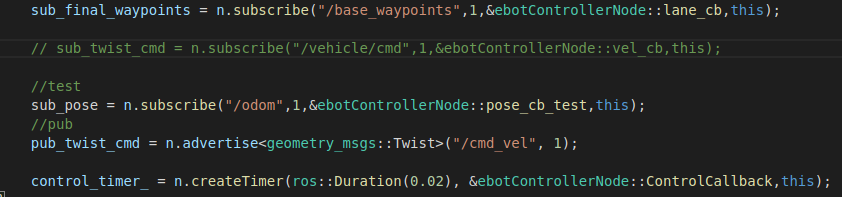
\includegraphics{figures/e2.png}
%     \caption{PID控制循迹}
% \end{figure} 
% 本来是输出图片,后面直接输出代码了
\begin{lstlisting}[style=whx]
    sub_final_waypoints = n.subscribe("/base_waypoints",1,&ebotControllerNode::lane_cb,this);

    // sub_twist_cmd = n.subscribe("/vehicle/cmd",1,&ebotControllerNode::vel_cb,this);

    //test
    sub_pose = n.subscribe("/odom",1,&ebotControllerNode::pose_cb_test,this);
    //pub
    pub_twist_cmd = n.advertise<geometry_msgs::Twist>("/cmd_vel", 1);

    control_timer_ = n.createTimer(ros::Duration(0.02), &ebotControllerNode::ControlCallback,this);
\end{lstlisting}

以此为例,第一个订阅sub\_final\_waypoints为接受的全局路径,这里我们接受的话题名字为/base\_waypoints,调用lane\_cb函数,得到路径信息。

第二个订阅sub\_pose接受车辆位姿,话题名为/odom,调用pose\_cb\_test函数来得到车辆位姿信息。

发布的话题为/cmd\_vel,与此相关的内容写在ControlCallback函数里面,以便周期调用发布,图例设置频率为50Hz(cpp中值设为0.02)。

修改好控制节点后,打开pid\_controller功能包下的CMakeList.txt,
在文件尾部可以看到add\_executable(**** src/****.cpp),target\_link\_libraries(**** \${catkin\_LIBRARIES})命令,
生成可执行文件。

可参照ros小乌龟例子,实现话题的发布与订阅。
https://blog.csdn.net/xtark\_robot/article/details/107860571

实验过程中,观察车辆偏离车道中心线的程度,以及车辆在循迹过程中是否快速、平稳。如果性能不尽人意需要及时调整相关参数。
\subsection{一些另外的调整}
\begin{enumerate}
    \item 将根目录下/src/vehicle\_sim/rviz/vehicle\_sim.rviz文件中keep参数设置为10000,keep=10000,保证小车全过程的轨迹线不消失。
    \item 编写python文件生成三种不同形状的轨迹路线,分别为方形,圆形,心形,以csv文件形式保存,方便后续调试。
    \item 生成路径时尽量使初始点位于原点即小车出发点;使设置路径的初始方向与小车开始方向一致,这样可以减少小车的转弯,更方便实验。
    \item 遵循一般的PID调参步骤,先调节P,再调节D,最后调节I。
    \item 每次调整完ebotController.cpp文件中的PID参数后,需要重新编译,否则不会生效。即需要运行\$catkin\_make 
\end{enumerate}

\section{实验结果}
初始PID参数为(0.4,0.3,0)

\subsection{直线轨迹}
\begin{figure}[H]
    \centering
    \begin{minipage}[t]{0.48\textwidth}
        \centering
        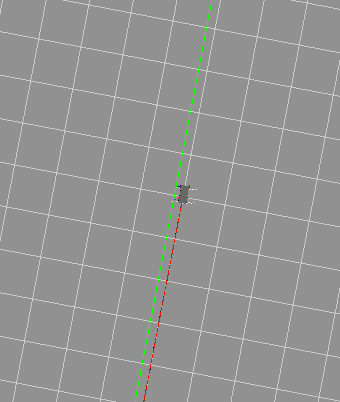
\includegraphics[width=0.8\textwidth]{figures/line000.png}
        \caption{直线轨迹0-0-0}
    \end{minipage}
    \begin{minipage}[t]{0.48\textwidth}
        \centering
        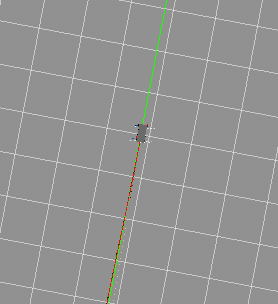
\includegraphics[width=0.8\textwidth]{figures/line300.png}
        \caption{直线轨迹0.3-0-0}
    \end{minipage}
\end{figure}
由上面两张图片可知,当P参数为0时,小车无法循迹;
当P参数为0.3时,小车能够正常循迹。

显示了P参数的循迹作用,根据误差的大小来控制输出,
让被控对象快速接近目标值。

\subsection{方形轨迹}

\begin{figure}[H]
    \centering
    \subfigure[方形轨迹0.4-0.3-0]{
        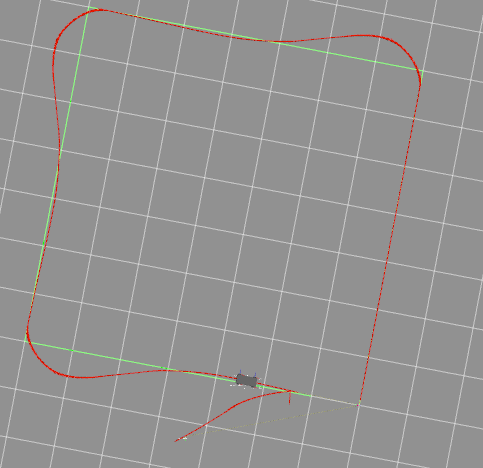
\includegraphics[width=2.5in]{figures/square430.png}
        \label{label_for_cross_ref_1}
    }
    \subfigure[方形轨迹0.6-0.3-0]{
	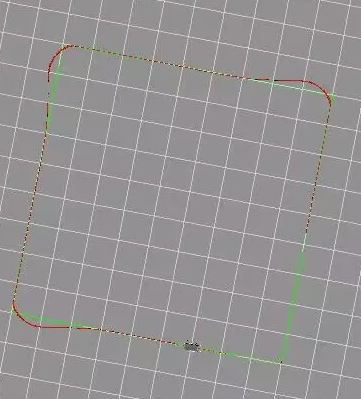
\includegraphics[width=2.5in]{figures/square630.png}
        \label{label_for_cross_ref_2}
    }
    \caption{方形轨迹}
\end{figure}
由上图可知,调大P参数能够使小车更加快速地循迹,
\subsection{圆形轨迹}

\begin{figure}[H]
    \centering
    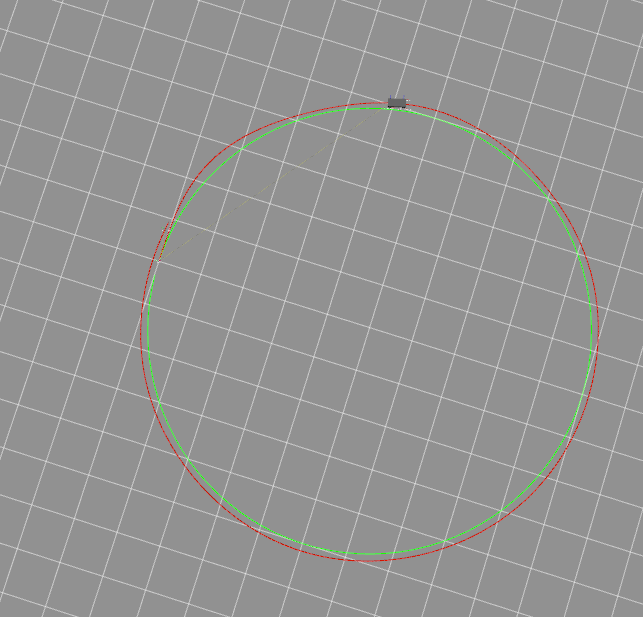
\includegraphics[width=2.5in]{figures/circle430.png}
    \caption{圆形轨迹0.4-0.3-0}
\end{figure}
默认参数已经可以较好地循迹,
但是小车绕圆运动时,运动半径总是大于圆半径,并难以消除误差。
后面发现在最后设定的PID参数下,小车几乎能够完美地绕圆运动。
\subsection{心形轨迹}

% \begin{figure}[H]
%     \centering
%     \begin{minipage}[t]{0.48\textwidth}
%         \centering
%         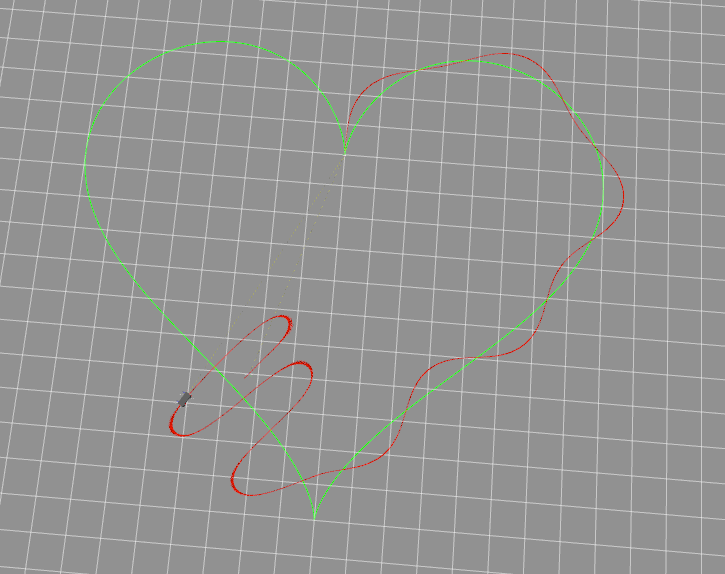
\includegraphics[width=0.8\textwidth]{figures/heart430.png}
%         \caption{心形轨迹0.4-0.3-0}
%     \end{minipage}

%     \begin{minipage}[t]{0.48\textwidth}
%         \centering
%         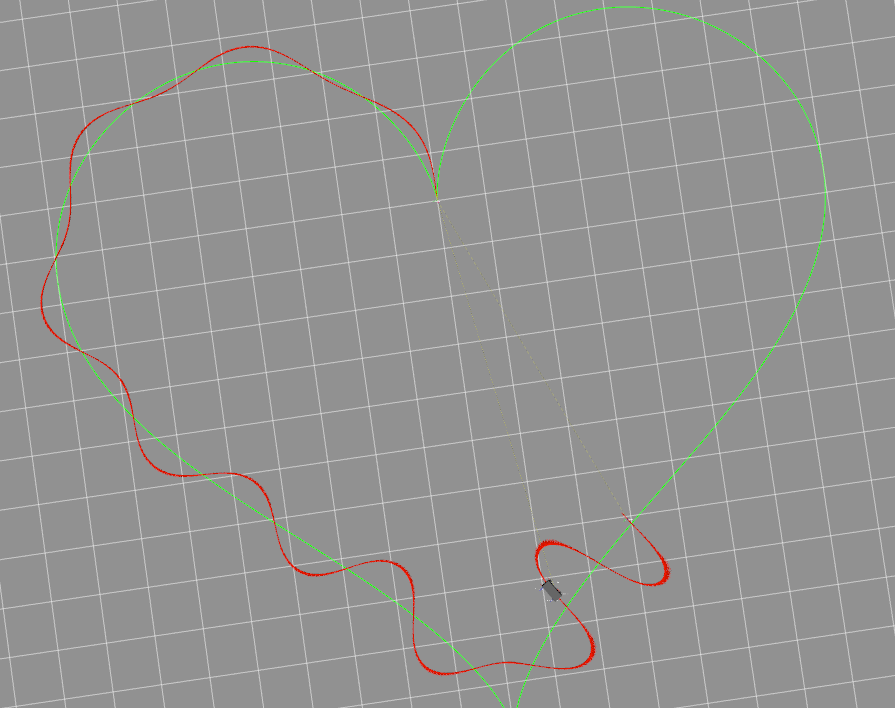
\includegraphics[width=0.8\textwidth]{figures/heart08030.png}
%         \caption{心形轨迹0.8-0.3-0}
%     \end{minipage}

%     \begin{minipage}[t]{0.48\textwidth}
%         \centering
%         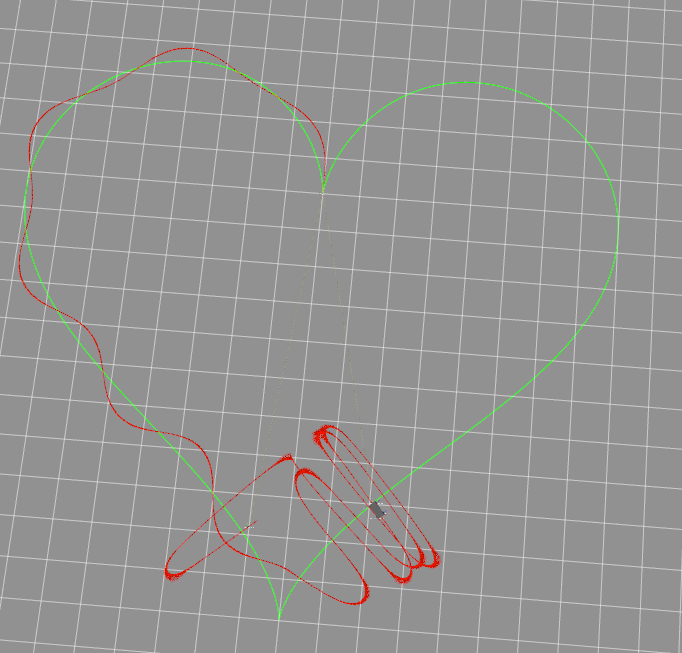
\includegraphics[width=0.8\textwidth]{figures/heart06010.png}
%         \caption{心形轨迹0.6-0.1-0}
%     \end{minipage}

%     \begin{minipage}[t]{0.48\textwidth}
%         \centering
%         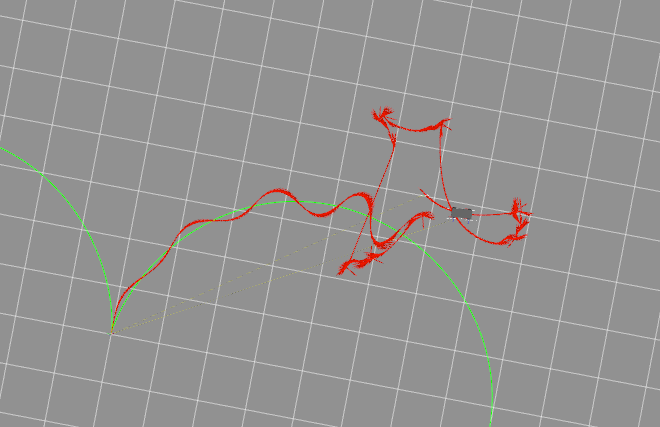
\includegraphics[width=0.8\textwidth]{figures/heart0603005.png}
%         \caption{心形轨迹0.6-0.3-0.5}
%     \end{minipage}
% \end{figure}
\begin{figure}[htbp]
    \centering
    \subfigure[心形轨迹0.4-0.3-0]{
        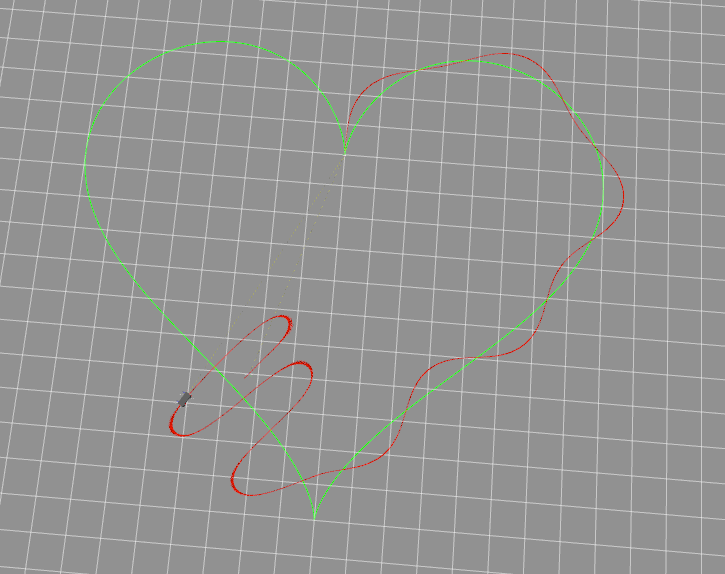
\includegraphics[width=2.5in]{figures/heart430.png}
        \label{label_for_cross_ref_1}
    }
    \subfigure[心形轨迹0.8-0.3-0]{
	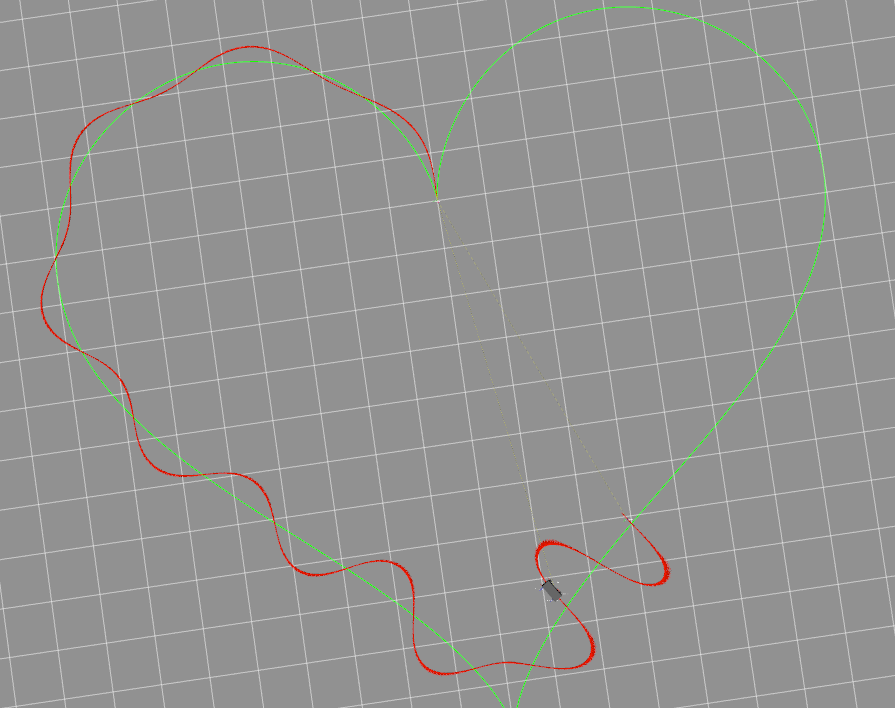
\includegraphics[width=2.5in]{figures/heart08030.png}
        \label{label_for_cross_ref_2}
    }
    % \quad    %用 \quad 来换行
    \\
    % 把\quad %用 \quad 来换行 换成 \\ 效果更好,否则图片尺寸太小时会在同一行
    \subfigure[心形轨迹0.6-0.3-0.05]{
    	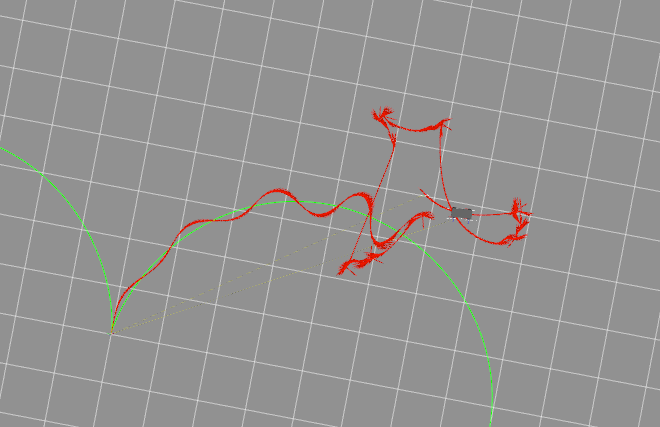
\includegraphics[width=2.5in]{figures/heart0603005.png}
        \label{label_for_cross_ref_3}
    }
    \subfigure[心形轨迹0.6-0.1-0]{
	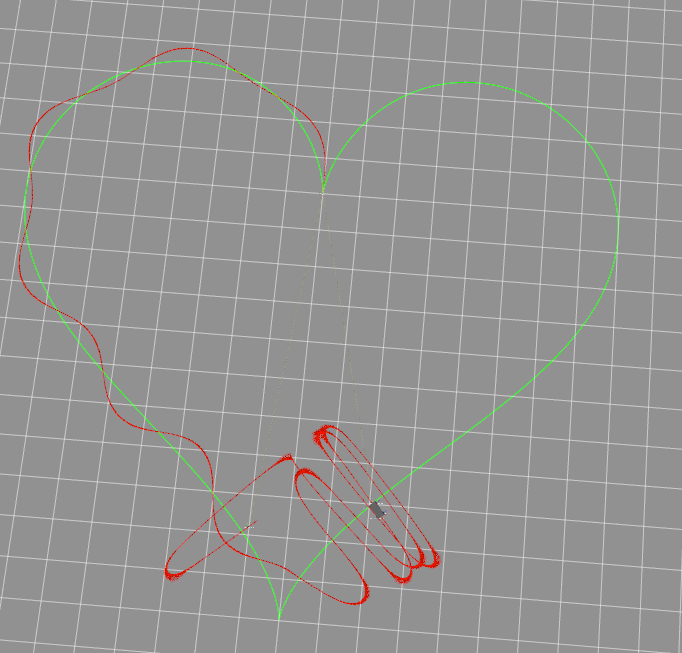
\includegraphics[width=2.5in]{figures/heart06010.png}
        \label{label_for_cross_ref_4}
    }
    \caption{心形轨迹}
    \label{fig.1}
\end{figure}
\begin{enumerate}
    \item 将心形线初始点坐标设为原点即小车出发点,并使初始曲线切向方向为小车运动方向,方便后续调节,也与现实条件相符。
    \item 小车初始向左转或者向右转均有可能发生,猜测是因为心形线取点个数不一样,导致初始曲线切向方向会有人眼无法识别的微小不同。
    \item 从图a我们可知,小车一开始能够在设定路径上摆动,进行效果较差的循迹,但是经过心形线的心尖处后,就会不断做椭圆的运动。
    \item 将图a至图b,发现调大P参数能够使小车更加快速地循迹,但是会增大初始误差,并难以消除;后续也无法突破转圈圈的问题。
    \item 从图b至图c,将参数P取成中间值0.6,参数I不变,参数D设置为0.05,但是小车在进行绕圆运动时就会出现偏离轨迹的情况。
    \item 从图d,我们将PID参数设置为0.6,0.1,0,发现仍然会出现经过心尖时后陷入椭圆运动的情况,而且比初始参数会更快地陷入困境。
\end{enumerate}

\begin{figure}[H]
    \centering
    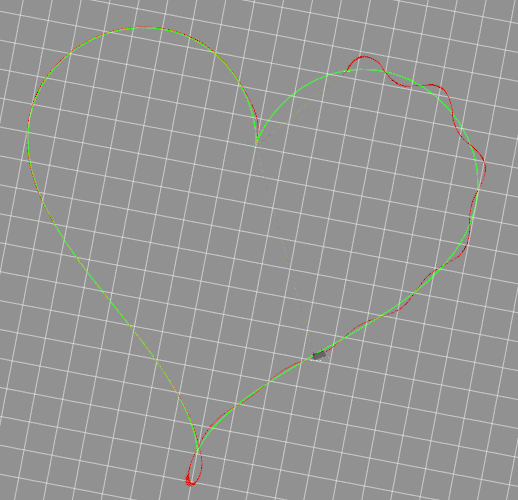
\includegraphics[width=0.7\textwidth]{figures/heart08001001.png}
    \caption{心形轨迹0.8-0.01-0.01}
\end{figure}
\begin{enumerate}
    \item 最后经过多次调参,发现将PID参数设置为0.8,0.01,0.01,小车能够在心形轨迹上进行完美的循迹。(即使增大I参数为0.2,似乎也能够很好地循迹)
    \item 小车经过心尖时,会画一个弧线后回到设定轨迹上。
    \item 美中不足的是,经过心尖后,小车似乎失去了原本能够完美拟合大弯曲线的能力,小车在结束点前的大弧线上运动时,会绕着设定轨道波动前进。
    \item 经过后续检验,此参数组在方形、圆形轨迹上都有几乎完美的循迹曲线。
\end{enumerate}

\section{总结分析}
\subsection{分析}
\begin{enumerate}
    \item 考虑心形线光滑度对小车循迹实验的结果
    
    首先,生成心形线轨迹的代码包含两个参数,a ,num\_points,后者的大小决定了心形线先的光滑度,越大,点越多,心形线轨迹越光滑。
    
    当路径上的点数量较少时,轨迹边界会显得比较粗糙,小车在进行路径跟踪时会出现较大的偏差,小车会进行多次钝角转弯,循迹效果可能会比较差。(参考矩形)

    相反,当路径上的点数量较多时,小车的循迹控制会更加精确和平稳,因为控制算法能够更精确地计算小车当前的位置和偏差。
    此外,路径上的点数量越多,小车与路径的误差就越小,因此可以实现更高的精度和稳定性。(参考圆形)

    但是,路径上的点数量过多也会导致问题。一方面,太多的点会增加算法的计算负担,导致实时性下降;
    另一方面,路径上的点数量过多会导致路径规划的复杂度增加,可能会导致路径规划算法无法在规定的时间内完成路径规划。

    因此,在确定路径上的点的数量时,需要权衡实时性、精度和计算负担等多个因素,并根据具体情况进行调整。
    故经过调试,我们选择了600个点作为最后的参数设置。(需要根据a和小车速度自行调节)

    \item 考虑PID参数调节方法
    
    在PID控制中,PID参数的合适取值需要根据具体的控制对象和控制要求来确定,通常需要通过试验和调整来得到。在一般情况下,可以按照以下步骤来设置PID参数:
    \begin{enumerate}
        \item 将三个参数(比例系数Kp、积分系数Ki、微分系数Kd)都设为0;
        \item 逐个增加参数,首先将Kp设为一个较小的值,然后观察系统响应,如果响应过度,可以逐渐减小Kp的值,直到响应合适;
        \item 在Kp合适的情况下,增加Ki的值,如果系统存在静态误差,可以通过增大Ki的值来减小误差,但是需要注意Ki过大会导致系统不稳定;
        \item 在Kp和Ki合适的情况下,增加Kd的值,可以通过增大Kd的值来减小系统的超调量,但是需要注意Kd过大会导致系统出现震荡;
        \item 可以通过反复试验和调整来得到合适的PID参数。
    \end{enumerate}
    需要注意的是,PID参数的取值不仅与控制对象和控制要求有关,还受到控制器的采样周期、噪声等因素的影响,因此在实际应用中需要进行更加细致和精确的调整。

\end{enumerate}

\subsection{总结}
在本次实验中,我们实现了基于PID的机器人循迹控制,并对不同算法进行了性能分析,并提出了改善控制性能的可行方案。

首先,我们通过使用网上文档、老师代码及指导书等资源创建工作空间并初始化,成功编译后,粗略地浏览控制代码并着重学习了重点部分代码。

其次,我们实现了基于PID算法的机器人循迹控制,该算法将误差的比例、积分和微分进行加权和计算,从而实现对被控对象的精确控制。在实验中,我们可以通过调整PID控制器中的三个系数,来获得较好的控制性能。

再次,经过多次调参,我们实现了对直线、方形、圆形、心形等轨迹的机器人循迹控制的PID参数调节,使机器人能够很好地以期望误差跟踪轨迹。

最后,我们通过对实验过程和实验图像的分析,总结了实验过程中的PID参数调节经验与方法。

\end{document}
